\documentclass[../main.tex]{subfiles}
\graphicspath{{\subfix{../Images}}}

\begin{document}
\section{Solidity Implementation in Ethereum Blockchain}
\label{sec:solidity_implementation}
\subsection{Introduction}
Ethereum is the most popular blockchain in academic research. Smart contracts were introduced with this blockchain, whose computation is delegated to the \textit{Ethereum Virtual Machine (EVM)}, essentially a distributed computing platform composed by the aggregated resources (CPU cycles, storage, memory, etc.) of the nodes that are active in the network at any point to run the computations required by smart contract function calls. This feature expanded the scope of usage of blockchain immensely and the academic community was quick to capitalise on it.
\par
The popularity of this chain warrants that we implement this system using a Solidity implementation, the programming language used to write Ethereum smart contracts, to both provide a standardised implementation and to serve as a baseline, since Solidity contracts have a more robust knowledge base than any other types, for future comparisons. This standardisation is achieved by implementing ERC standards in the contracts that establish the framework for this system.
\par
Solidity implements NFTs in a non-structured fashion, in the sense that these are not digital objects from a programming standpoint. Solidity NFTs are not like typical digital objects from any Object-Oriented programming language, which are defined by internal parameters and functions. In Solidity, any NFT parameters are established by mapping the unique NFT identifier to another variable (integer, url string, address, etc.) and the collection of all these mappings with the same id key compose the actual NFT object. Functions are defined in the same smart contract that defines the NFT, so these are not necessarily NFT functions, as some languages allow objects to have. These functions may be limited to operate on NFT-defining mappings, thus restricted to operate on NFT data, but they belong to the containing contract and have no logical relation with the NFTs themselves.
\par
Due to the lack of specificity in Solidity NFTs, as in they do not carry a data type themselves, from this point forward we designate the NFTs used to carry the votes as \textbf{VoteNFT}.

\subsection{Smart Contract Implementation}
The main voting contract was defined to emulate a voting booth. Like one, this contract can give a ballot to a voter as a NFT transfer to the voter address, allow the voter to vote by changing a parameter in the VoteNFT metadata to his or her choice and even burn the voteNFT.
\par
The vote function also allows for multiple vote casting, i.e., after submitting a vote, if the election is still active, the voter can submit another voteNFT at a later stage and this one replaces the previous one. From this implementation point of view, the voter only edits the same NFT field again, since it is a more practical and cheaper (gas wise) alternative to burn the old VoteNFT, mint a new one and run the vote function again. Additional edits are protected against unauthorised uses like the initial vote.
\par
If a voter can replace a vote, he/she should also be able to revoke it. This feature is established by a 'burn' function that adds more requirements for its execution, but otherwise it is inherited from the \textit{ERC721Burnable} standard implemented, i.e., it transfers the VoteNFT to address 0.

\subsubsection{ERC Standards Used}
The voting booth smart contract implements the base \textit{ERC721} standard that implements the majority of internal mappings that define our VoteNFT, as well as useful functions such as \textit{balanceOf} and a base NFT minting function. This standard can be expanded with other \textit{ERC721} based "sub-standards", i.e., standards based on the \textit{ERC721} that add new functionalities to a NFT implementation. The \textit{ERC721URIStorage} and \textit{ERC721Burnable} were added to the base \textit{ERC721} standard. The \textit{Burnable} extension adds the \textit{burn} function and the \textit{URIStorage} extension includes a id to string mapping that we use to encode the vote, but it is often used to write a URL that points to the "actual" digital object abstracted by the NFT (image, video, audio clip, etc.). This standard also exposes a \textbf{\_setTokenURI} internal function that can be used to modify the NFT metadata towards our goals.

\subsubsection{Using \textit{balanceOf} to Ensure One Person, One Vote}
A fundamental requisite for any voting system, electronic or otherwise, is to allow one and only one vote per eligible voter. This is actually a fundamental requirement from representative democracies, and not necessarily from the systems used to capture those votes. It is important to note that this requirement does not conflict with the \textit{multiple vote casting} feature nor with the ability of a voter to revoke an already submitted vote. Allowing voters to cast multiple votes does not violates the "one person, one vote" rule, as long as only one of those submission ends up in the final tally (usually the last one submitted). The same logic stands with allowing votes to be revoked, in the sense that submitting zero votes is also a valid scenario for a voter.
\par
The \textit{ERC721} standard provides a \textit{balanceOf} function that receives an argument as input and returns the number of NFT tokens that are defined in the contract instance that are owned by such address. This function returns the value of one of the \textit{ERC721} internal mappings, namely the \textbf{\_balances} one, associated to the address key. By ensuring that this field can only be 0 or 1, the system ensures that no voter can hold more than 1 VoteNFT at any point in the process. Since this function is made available by implementing the interface and it does exactly what it is required to implement this requirement, no additional functions were created and this one is used whenever this verification is necessary.
\par
The \textit{ERC721} standard ensures that, as long as one uses the functions inherited from the standard to operate on NFTs, namely, minting and transfers, the internal \textbf{\_balances} mapping is always updated correctly. With that in consideration, we employ functions from the implemented standards as close to their original and tried format as possible. Also, all alterations included when overriding one of these standardises functions do not interfere in any capacity with this mapping.

\subsubsection{The VoteNFT}
\paragraph{Mappings}
\label{sec:mappings}
Solidity defines NFTs as an aggregate of mappings that establish relationships between a unique identifier in the NFT and other parameters. NFTs are defined in Solidity in a similar fashion as centralised databases work, namely, how a  database is usually spread through multiple tables that maintain relationships between their records, typically by having sharing one or more columns in common. The full set of parameters that define a NFT are found by retrieving every mapping record that references the unique NFT identifier. These mappings include all defined in the original smart contract and any inherited from implementing standards.
\par
As such, the proposed implementation for this token can be explained by the mappings that compose it. Fig. \ref{fig:votenft_mappings} identifies these mappings as well as their origin, i.e., if these were inherited from one of the standards implemented or if they were created in the NFT smart contract.

\begin{figure}[htp]
    \centering
    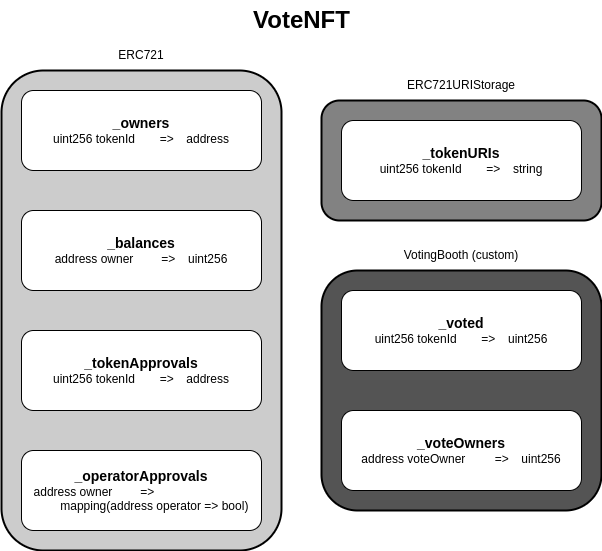
\includegraphics[width=0.7\textwidth]{../Images/01_VoteNFT_Mappings.png}
    \caption{Mappings used to implement the Solidity version of VoteNFT.}
    \label{fig:votenft_mappings}
\end{figure}

The mappings that establish the base definition of this token are all inherited from the \textit{ERC721} standard, namely the \textbf{\_owners} and \textbf{\_balances}, which are used to establish the ownership of the issued tokens and to ensure that only one token gets owned per voter.
\todo{This next part might need revision in the future, if I decide to use this mappings to change the whole token access logic}
The \textbf{\_tokenApprovals} and \textbf{\_operatorApprovals} are used to add two layers of access control to the tokens produced by the contract. These can be used to delegate access to a minted token to accounts other than the owner. This is antithetical to the purpose of the vote tokens, therefore these are not currently used. In fact, having any data in either of these mappings might be interpreted as a security risk since they might allow access to accounts other than the one from an eligible voter, which can be used to modify the voteNFT data after the owner has done so, for example. These mappings are all inherited from the \textit{ERC721} standard.
\par
The \textit{ERC721URIStorage} standard provides the \textbf{\_tokenURIs} mapping that is used to store the ballot contents. Most NFTs so far use this field to set an URL pointing to the digital resource that characterises the NFT (an image, video or audio clip) but in this case we used it to encode the voter option. This way, all the information regarding the vote remains in the blockchain, therefore it enjoys all the data immutability and transparency from having this data distributed through a series of nodes in the network. Setting a URL to a proxy server where the actual ballot is negates this entirely and it is a major security breach since it introduces an external element to the blockchain network. Realistically, the final tally for a particular smart contract can be computed by reading and counting all the values in this mapping since all the data needed to determine the winner is contained in this mapping.
\par
The mappings inherited from the standards are sufficient for most of what is needed, but to ease some operations, two extra, custom mappings were added to the VoteNFT smart contract, namely, the \textbf{\_voted} and \textbf{\_voteOwners} mappings. \textbf{\_voted} maps the token's unique identifier to another integer that represents the number of times that the metadata of the VoteNFT with the id in question was edited after minting, which in this context means a new vote being submitted. This mapping is only being used to detect if a voter is voting for the first time (\_voted[tokenId] = 0) or if the voter is replacing a previously submitted vote (\_voted[tokenId] >= 1) and, so far, it is being used to determine which event should be emitted, namely the \textit{VoteSubmitted(voteId)} event or the \textit{VoteModified(voteId)} event. These events signal that a vote with a specific id was submitted or modified but without revealing any more information about it than the id of the token itself. The \textbf{\_voteOwners} mapping is a simple inversion of the \textit{ERC721} \textbf{\_owners} one. It maps the owner address to the id of the VoteNFT awarded to him/her and it is used to provide redundancy to the \textbf{\_balances} mapping in the sense that locks one address to one voteId (Solidity mappings, just like dictionaries in other programming languages, do not allow duplicate keys) more strictly than using the \textbf{\_balances} mapping alone. It also provides a easier and cheaper (gas wise) way to determine if a user address already has a token issued to it. Without this mapping, the only process to determine this is to exhaustively check every value from the \textbf{\_owners} mapping, which can be a very time and gas expensive operation.

\paragraph{Relevant Contract Functions}
Alongside the mappings indicated in Section \ref{sec:mappings}, the VotingBooth smart contract contains a series of functions used to operate in the NFTs created by the same contract:

\begin{itemize}
    \item {\textit{Constructor} The constructor function for the VotingBooth smart contract, not the VoteNFT. The constructor in a smart contract is a function that runs once when the contract is deployed. It can take input arguments but once the contract is deployed, this function never runs again. The constructor does not influence the VoteNFT tokens, but it is used to define the election in question by establishing internal contract parameters such as the name and location, as well as the ballot string, i.e., the list of candidates in play, a referendum question, etc.}
    \item {\textit{mintVoteNFT} The minting function to generate a VoteNFT. DMinting VoteNFTs is a critical operation in this system. As such, this function can only be executed by the contract deployer. If a transaction signed by another account other than the one that deployed the contract, a requirement at the top is going to prevent it from continuing if the field \textit{msg.sender} does not matches the allowed address. The function sets the sole input argument, an address, as the NFT owner. Minting a VoteNFT consists in taking an internal counter value as the id for the token that is about to get created, and then proceeds by using that id to create a record into the mappings indicated in Fig. \ref{fig:votenft_mappings}. The function finishes by incrementing the internal counter for the next mint call and emitting the event that signals a successful minting.}
    \item {\textit{vote} Similar to the minting function, the vote function is also limited to the owner of the NFT and validates this requirement using a similar requirement at the top. Only transactions signed by an address that matches the address in the \textbf{\_owners} mapping for the id in question is allowed to proceed. If this validation is cleared, the function replaces the contents from the \textbf{\_tokenURIs} mapping for the string provided as input. If this modification is the first one after minting, the action is assumed as vote. Otherwise it is assumed as a replacement vote. The function finishes by emitting a \textit{VoteSubmitted} or \textit{VoteModifies} event accordingly}
    \item {\textit{burn} This function removes a VoteNFT from circulation by transferring it to an unrecoverable address. Voters have the option to revoke a previously submitted vote without requiring to provide a substitution one. In these cases, the \textit{burn} function is executed instead. Burning a VoteNFT is restricted to the token owner as well and a \textit{VoteBurned} event gets emitted when the function terminates successfully.}
\end{itemize}

\subsection{Usage example}


\todo{Encryption layer}
\todo{Tally contract}
\todo{Eligibility step}
\todo{Setup the gas reporter}
\todo{How to rewrite the 'vote' function to limit options, validate the ballot and detect invalid options?}
\todo{Should we add the Solidity code as annex? Inline?}

\end{document}
